\documentclass{article}
\usepackage[utf8]{inputenc}
\usepackage{eurosym}
\usepackage{natbib}
\usepackage{graphicx}
\usepackage[a4paper,left=2cm,right=2cm,top=2cm,bottom=2cm]{geometry}
\usepackage[french]{babel}
\usepackage[T1]{fontenc}
\usepackage[linktoc=all,pdfpagemode=UseNone]{hyperref}
\usepackage{verbatim}
\usepackage{array}
\usepackage{hhline}
\usepackage[justification=centering,margin=2cm]{caption}
\usepackage{subcaption}
\usepackage{rotating}

%\hypersetup{
    %colorlinks,
    %citecolor=black,
    %filecolor=black,
    %linkcolor=black,
    %urlcolor=blue
%}	
%\newenvironment{desc}{\textit\bgroup}{\egroup} % Description des parties visibles (en italique)
\newenvironment{desc}{\comment}{\endcomment} % Description des parties invisible

% Redéfinie les sections pour leur donner une indentation
\makeatletter
\renewcommand\section{\newpage
																	 \@startsection{section}{1}{\z@}
                                   {-3.5ex \@plus -1ex \@minus -.2ex}
                                   {2.3ex \@plus.2ex}
                                   {\normalfont\Large\bfseries}}
\renewcommand\subsection{\@startsection{subsection}{2}{5ex}
                                     {-3.25ex\@plus -1ex \@minus -.2ex}
                                     {1.5ex \@plus .2ex}
                                     {\normalfont\large\bfseries}}
\renewcommand\subsubsection{\@startsection{subsubsection}{3}{10ex}
                                     {-3.25ex\@plus -1ex \@minus -.2ex}
                                     {1.5ex \@plus .2ex}
                                     {\normalfont\normalsize\bfseries}}
\makeatother

% Renumérote les sections en I 1 a
\renewcommand{\thesection}{\Roman{section}.}
\renewcommand{\thesubsection}{\thesection\arabic{subsection}.}
\renewcommand{\thesubsubsection}{\thesubsection\alph{subsubsection}.}

\begin{document}

\pagenumbering{gobble}
\begin{titlepage}
	\newcommand{\hsp}{\hspace{20pt}}
	\newcommand{\HRule}{\rule{\linewidth}{0.5mm}}
  \begin{sffamily}
  \begin{center}

		\begin{tabular}{p{0.35\textwidth} p{0.65\textwidth}}
			\begin{center}\vspace{0pt} 
\includegraphics[width=0.25\textwidth]{logo-lip6.png}\end{center} &
			\begin{center}\vspace{0pt} 
\includegraphics[width=0.55\textwidth]{logo-upmc.png}\end{center}
		\end{tabular}
		
	
		~\\[2cm]

    

    % Title
    \HRule \\[0.4cm]
    { \huge \bfseries Provisionnement dynamique de serveurs de jeux massivement multijoueurs\\[0.4cm] }

    \HRule \\[3cm]
		
		\textsc{\LARGE Stage Master 2\ieme{} année}\\[0.5cm]

    \textsc{\Large Rapport bibliographique}\\[4cm]

    % Author and supervisor
    \begin{minipage}{0.4\textwidth}
      \begin{flushleft} \large
        Guillaume \textsc{Turchini}\\[0.5cm]
				\textbf{\emph{Rapporteur :}} M.~Julien~\textsc{Sopena}
      \end{flushleft}
    \end{minipage}
    \begin{minipage}{0.4\textwidth}
      \begin{flushright} \large
				\textbf{\emph{Tuteurs :}} Mme.~Maha~\textsc{Abdallah} M.~Olivier~\textsc{Marin} M.~Sébastien~\textsc{Monnet}
      \end{flushright}
    \end{minipage}

    \vfill

    % Bottom of the page
    {\large Mars - Août 2015}

  \end{center}
  \end{sffamily}
\end{titlepage}


\tableofcontents

\section{Introduction}
\pagenumbering{arabic}
\`A l'origine, les jeux en ligne permettaient à un nombre limité de joueurs (usuellement 16 voir 64) de se rencontrer dans des parties relativement courtes.
De nos jours, de plus en plus de jeux massivement multijoueurs en ligne (MMOG) permettent à des milliers de joueurs de se rencontrer dans un univers persistant.
Le genre a été popularisé à la fin des années 1990 par la sortie de MMORPG (jeux de rôle massivement multijoueurs en ligne) tels que ``Ultima Online''~\cite{ultima_online}, ``Lineage''~\cite{lineage} ou ``Everquest''~\cite{everquest}.
En 2004, Blizzard Entertainment a sorti ``World of Warcraft'' (WOW)~\cite{wow} qui a eu immédiatement un grand succès et qui continue aujourd'hui à être un des plus grands MMORPG avec encore près de 10 millions d'utilisateurs dans le monde fin 2014~\cite{wow_player_num}.

Les serveurs de ces jeux doivent servir un très grand nombre de joueurs connectés (habituellement plus de 1000 joueurs) en leur délivrant une vue cohérente tout en gardant une expérience de jeu agréable, ce qui signifie avoir des temps de réponse acceptables la plupart du temps~\cite{latency_can_kill}.
Un serveur ne peut gérer qu'un nombre fini de joueurs car il est limité par sa puissance.
Il est donc nécessaire de partitionner le serveur.
L'intérêt de cette capacité à tenir la charge induite par de nombreux joueurs est important au lancement d'un jeu car le succès d'un jeu se fait bien souvent par la première expérience des joueurs.
Il est donc nécessaire d'avoir suffisamment de marge au niveau du nombre de joueurs côté serveur pour ne pas être surchargé.
La solution utilisée par les industriels est donc de surdimensionner l'architecture serveur.
Cependant il faut faire attention à ne pas surdimensionner l'architecture sous peine de dépenser tous les profits du jeu.

Les jeux fortement anticipés ne supportent souvent pas le pic de charge induit par le nombre de joueur voulant se connecter au lancement du jeu.
De même, si de nombreux joueurs décident de se réunir à un même endroit, où l'architecture n'est pas prévue pour en supporter autant, le serveur de jeu crash.
Certains jeux supportent ce grand nombre de joueurs par le design du jeu.
Par exemple, Dragon Quest X, qui peut supporter aux environs de 300 000 joueurs concurrents, réduis les interactions possibles entre les joueurs.
Les groupes sont composés de 4 joueurs maximum et il n'est que possible d'encourager les autres groupes de joueurs.
Cela réduit la contrainte de temps nécessaire au transfert de l'information des joueurs, l'interaction n'étant pas critique.
Par la suite, ce rapport s'intéresse donc aux jeux ayant un grand nombre de joueurs et une forte interaction entre eux, imposant des temps de réponses stricts.

Dans la suite de ce rapport, nous appellerons ``serveur'' l'entité hébergeant le monde du jeu dans sa globalité.
Les serveurs des jeux s'exécutent soit directement sur une ou plusieurs ``machine(s)'' physique(s), soit sur des ``machines virtuelles'' (VM) hébergées dans un cloud.

Nous détaillerons dans la partie II de ce rapport les différentes méthodes de partitionnement qui sont utilisées actuellement pour répondre aux problèmes de passage à l'échelle.
Dans la partie III, nous présenterons les différentes architectures pour héberger les serveurs de jeu se basant sur ces partitionnements.
Ensuite, nous verrons en partie IV les métriques permettant de comparer ces architectures à notre solution.
Nous présenterons dans la partie V la simulation de l'architecture.
Enfin, nous conclurons dans la partie VI sur les enjeux à venir et les algorithmes à tester.


\section{Partitionnement du serveur}
Un serveur de jeu vidéo classique ne peut gérer qu'un nombre fini de clients. Cependant, les MMOG d'aujourd'hui dépassent largement ce nombre et doivent donc utiliser des méthodes permettant le passage à l'échelle. Pour ce faire, ils partitionnent le serveur de jeu pour lui permettre d'être exécuté sur plusieurs machines.\\

Dans cette partie, nous allons présenter les différentes stratégies de partitionnement utilisées dans les serveurs de jeux vidéos actuels. Ces solutions peuvent être combinées, toutes les combinaisons sont possibles, y compris toutes les solutions en même temps.

\begin{figure}[b!]
	\centering
	\begin{sideways}\qquad\quad~Nombre de joueur\end{sideways}
	\begin{subfigure}[b]{0.5\textwidth}
		\centering
		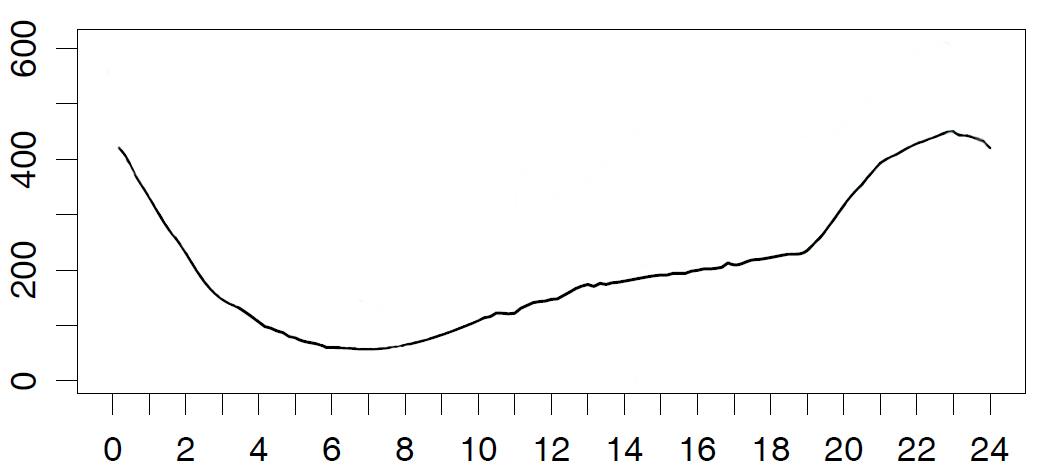
\includegraphics[width=\textwidth]{player_day_evol.png}\\
		Heure
	\end{subfigure}
	\\[0.2cm]
	\caption{Evolution du nombre moyen de joueurs au cours d'une journée sur un royaume de World of Warcraft entre Janvier et Septembre 2006 (voir~\cite{is_server_consolidation_benefical})}
	\label{fig:player_day_evol}
\end{figure}

\subsection{Mouvements des joueurs}
Une des difficultés du partitionnement d'un serveur de MMOG est que la population de ces jeux évolue au cours du temps, à la fois en nombre et en répartition.\\

Comme indiqué dans la \textsc{Figure}~\ref{fig:player_day_evol}, le nombre de joueurs connectés à un serveur jeu varie grandement au cours du temps~\cite{is_server_consolidation_benefical}. En effet, dans une même journée, la période de haute affluence se situe aux alentours de 23h et celle de basse affluence aux alentours de 7h du matin. Ceci s'explique par le fait que les joueurs se connectent en rentrant du travail après le repas et se reposent la nuit. On peut également remarquer que le nombre de joueurs varie aussi au cours de la semaine. Les samedis et dimanches, on observe en moyenne plus de joueurs en globalité (mais un pic maximal identique). Cette variation de joueurs peut entraîner le crash d'un serveur de jeu. On peut observer ce phénomène le premier jour d'un jeu attendu, l'architecture étant totalement saturée par les personnes se connectant à l'heure de sortie du jeu.\\

Il est facile de comprendre dans le cas d'un jeu vidéo qu'il y ait des zones du jeu plus prisées que d'autres. En effet, il existe souvent un but au jeu et les objectifs attirent donc naturellement plus de monde. Dans un MMORPG, les zones correspondant aux villes (qui sont généralement les zones de sociabilisation) et les zones correspondant aux objets les plus rares et puissants sont considérées comme des ``hotspots'' (points chauds) qui correspondent à des centres d'attraction de joueurs. La majeure partie du temps le reste du monde en dehors de ces hotspots reste plutôt vide. Un exemple de ce type de répartition est donné en \textsc{Figure}~\ref{fig:partitionnement_mono}.\\

Ces paramètres variant beaucoup au cours du temps, il faut que le partitionnement puisse s'adapter à ces changements pour être efficace.

\subsection{Séparation des services}
Le but de ce type de partitionnement est de séparer les entités distinctes de l'architecture d'un serveur de jeu vidéo. Les entités usuelles d'un serveur sont:\\

\begin{itemize}
	\item La couche de persistance (usuellement une base de données) qui permet de stocker l'état du jeu.
	\item La couche d'authentification qui permet aux joueurs de se connecter avec leurs identifiants.
	\item La couche logique de jeu qui constitue le traitement des déplacement des éléments du jeu.
	\item La couche service permettant aux administrateurs système d'observer les serveurs (statistiques).\\
\end{itemize}

Cette liste n'est pas exhaustive et n'est pas non plus une liste d'éléments obligatoirement présents sur un serveur de jeu. Cette séparation permet d'éviter d'exécuter toutes les applications sur une même machine et donc qu'une application ne surcharge le processeur et ni n'en pénalise une autre. Elle permet également de mettre en place des techniques de duplication (mirroring) de la base de données pour gérer plus de lectures parallèles. Cela est typiquement utilisé conjointement à un autre partitionnement, par exemple une séparation par zone (voir partie suivante), en utilisant un réplicat par zone.

\begin{figure}[b!]
	\setlength{\fboxsep}{0pt}
		\centering
		\begin{subfigure}[t]{0.22\textwidth}
		\vspace{0pt}
			\framebox{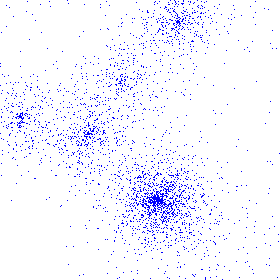
\includegraphics[width=\textwidth]{nuage_mono.png}}
			\caption{Exemple de répartition de la population}
			\label{fig:partitionnement_mono}
		\end{subfigure}
		~
		\begin{subfigure}[t]{0.22\textwidth}
		\vspace{0pt}
			\framebox{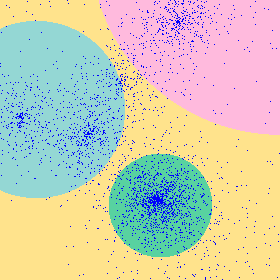
\includegraphics[width=\textwidth]{nuage_zonage.png}}
			\caption{Zoning}
			\label{fig:partitionnement_zonage}
		\end{subfigure}
		~
		\begin{subfigure}[t]{0.22\textwidth}
		\centering
		\vspace{0.5cm}
			\begin{tabular}{*{2}{>{\centering\arraybackslash}m{0.4\textwidth}}}
				\multicolumn{2}{c}{\framebox{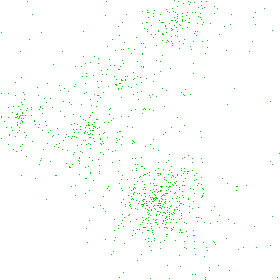
\includegraphics[width=0.4\textwidth]{nuage_sharding_vert.png}}}\\
				\framebox{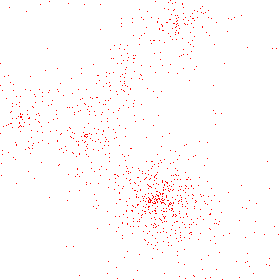
\includegraphics[width=0.4\textwidth]{nuage_sharding_rouge.png}}&
				\framebox{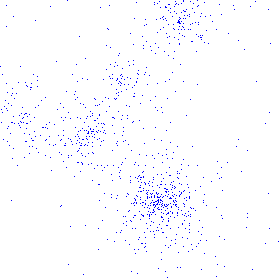
\includegraphics[width=0.4\textwidth]{nuage_sharding_bleu.png}}
			\end{tabular}
		\caption{Sharding}
		\label{fig:partitionnement_sharding}
		\end{subfigure}
		~
		\begin{subfigure}[t]{0.22\textwidth}
		\vspace{0pt}
			\framebox{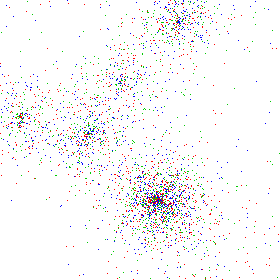
\includegraphics[width=\textwidth]{nuage_cloning.png}}
			\caption{Clonage}
			\label{fig:partitionnement_clonage}
		\end{subfigure}
		\\[0.2cm]
	\caption{Types de partitionnement}
	\label{fig:partitionnement}
\end{figure}

\subsection{Zoning}
Le zoning correspond au découpage du monde du jeu en différentes zones qui peuvent être gérées par des machines différentes, une machine étant donc responsable d'une ou plusieurs zones (voir \textsc{Figure}~\ref{fig:partitionnement_zonage}). Ces zones sont souvent séparées par des limites géographiques dans le monde du jeu (montagnes, rivières, mers...) et sont donc souvent fixes. Les zones ne sont généralement pas transparentes pour les joueurs, ce qui réduit l'immersion dans le jeu car elles sont accompagnées de zone de chargement dans le jeu et l'interaction de deux joueurs à la frontière n'est pas possible.\\

Pour contrer le problème des interactions aux frontières, des techniques de synchronisations inter-serveur peuvent être mises en places pour avoir l'illusion d'un monde sans frontière. Cette solution apporte cependant un coût et une complexité plus élevés. Une méthode pour gérer ce problème est la création de zone de chevauchement (overlap) dont les objets sont gérés par les deux machines en même temps.\\

Les zones étant fixes, un grand nombre de joueurs peut se retrouver dans une même zone et entraîner une surcharge de la machine responsable de cette zone. Pour contrer ceci, on peut partitionner le monde en micro-zones et répartir celles-ci dynamiquement entre les machines du serveur~\cite{triangle_based_load_balancing}. Les micro-zones peuvent également être dynamiques pour être sûr de ne pas en surcharger une. Ceci complexifie les interactions aux frontières car l'architecture est fortement dynamique. Cette solution vient avec un coût de transfert qui peut totalement contrebalancer les bénéfices de cette méthode, voire pénaliser son utilisation, surtout si les zones sont très petites et les transferts nombreux.\\

Cette dernière méthode de partitionnement fonctionne bien mais est complexe. Le zoning est le partitionnement principal de l'architecture que nous allons proposer en partie IV car celui-ci ne sépare pas les joueurs en groupes ne pouvant pas interagir. Ce domaine reste encore un sujet ouvert de la recherche car il est nécessaire de trouver de bons algorithmes permettant le dynamisme des zones.

\subsection{Sharding}
Plutôt que de séparer le monde du jeu en plusieurs zones, cette technique consiste à dupliquer le monde du jeu et à répartir la masse de joueurs en plusieurs groupes qui seront hébergés sur différentes machines ayant chacun une copie du monde du jeu (voir \textsc{Figure}~\ref{fig:partitionnement_sharding}). La majeure partie des MMOG utilisent cette technique en nommant ces groupes shards, royaumes (realm) ou mondes (world). Chaque monde est indépendant et ne peut communiquer. La charge des serveurs est limitée en diminuant le nombre maximum de joueurs par monde. Il suffit ensuite d'ajouter ou de retirer des mondes selon le nombre de joueurs, telles des tables de poker dans un casino. Cependant, tout comme les tables de poker, les joueurs ne jouent pas réellement ensemble.\\

Cette approche sépare les joueurs et limite donc les interactions inter-joueurs à ceux se situant dans le même monde, cette séparation étant souvent fixe. Dans World of Warcraft par exemple, avant la création d'un avatar, il faut choisir le royaume dans lequel on souhaite jouer. Cependant, des options de migrations sont actuellement disponibles dans World of Warcraft pour passer d'un royaume à un autre, coûtant 20\euro{} pour une migration vers n'importe quel serveur et gratuite pour passer d'un serveur à population élevé vers un serveur à population faible. Le prix ne sert pas ici à faire des bénéfices mais à équilibrer la charge entre les serveurs.

\subsection{Instancing}
Cette solution se situe à mi-chemin entre les deux solutions précédentes. Une instance est une copie d'une zone et il peut exister plusieurs copies d'une zone. Un joueur peut interagir avec les autres joueurs de cette instance mais pas avec les joueurs d'une autre instance de cette même zone. Chaque instance hébergeant un nombre limité de joueurs, la charge générée par une unique instance n'est pas grande et plusieurs instances peuvent être attribuées à une seule machine. Elles peuvent également être distribuées dynamiquement entre les machines.\\

Certains joueurs peuvent donc se donner rendez-vous et se retrouver au même endroit sans se voir, ce qui réduit l'immersion du joueur. Dans la plupart des jeux, seules des zones réduites sont instanciées. Celles-ci se font en groupes de joueurs s'étant organisés avant de pénétrer dans la zone instanciée. Ces zones sont la plupart du temps ce qui est appelé ``donjon'' dans les jeux de rôles (endroits fermé). Cela permet à chaque groupe de joueurs d'expérimenter le même contenu au même moment sans subir les interférences d'un autre groupe et cette séparation, bien que nuisant à l'immersion, est donc nécessaire pour des questions de jouabilité.\\

Certains jeux instancient les zones d'affluence telles que les villes et capitales. Cependant, il est dans ce cas souvent possible de changer d'instance à la volée à la demande du joueur pour rejoindre un camarade de jeu par exemple.

\subsection{Autres techniques}
D'autres techniques utilisées sont plus rarement observées.
\paragraph{Clonage\\}
Cette technique répartit le coût du calcul des actions des joueurs sur plusieurs machines gérant conjointement la même zone. Dans certains jeux comme les jeux de stratégie en temps réel (RTS), des calculs sont à effectuer lors d'un clic de déplacement d'un joueur, comme calculer le chemin que vont prendre les unités (pathfinding) ou le déplacement en formation des unités. Ces calculs étant plus lourds, chaque machine est en charge d'un ou plusieurs joueurs et effectue les calculs en parallèle (voir \textsc{Figure}~\ref{fig:partitionnement_clonage}). En cas d'interaction entre deux joueurs n'étant pas gérés par la même machine, il faut mettre en place des mécanismes de verrou de modification pour éviter d'arriver à des résultats incohérents.
\paragraph{Ralentissement du temps\\}
Cette technique consiste à ralentir le déroulement du temps sur le serveur pour permettre au serveur de traiter toutes les actions et de les transmettre aux joueurs. Ainsi le temps entre deux mises à jour pour le client est ralenti. Cette solution est utilisée dans le jeu Eve Online pour les combats de vaisseaux de grande ampleur où la gestion des collisions entre vaisseaux et missiles ainsi que les mouvement des joueurs devient très intensive pour une même zone. Il faut bien sûr remarquer que ce type de solution n'est pas envisageable dans n'importe quel type de jeu car les mécaniques du jeu ne s'y prêtent pas forcément. Par exemple, un jeu de tir à la première personne (FPS), basé sur les réflexes, nécessite des actions rapides. Dans ce cas, ce genre de solution n'est pas utilisable.

\subsection{Conclusion}
La mise en place de ces techniques de partitionnement par les développeurs de MMOG montre qu'il existe un réel problème de passage à l'échelle. Dans la majorité des cas, l'ensemble des joueurs est séparé en plus petits groupes pour limiter le nombre de joueurs en interaction. Cela permet de ramener le nombre de joueurs à un nombre pouvant être géré par les architectures existantes décrites en partie III. Ceci montre qu'il y a donc un besoin en solutions permettant à tous les joueurs de jouer réellement ensemble.


\section{Architectures se basant sur ces partitionnements}

\subsection{Principales problématiques}
Bien que la première partie de ce rapport ait exposé des pistes de résolution du problème de la charge d'une seule machine, d'autres problématiques complexes se posent sur la gestion d'un serveur de jeu vidéo.

\paragraph{Division du monde entre les machines\\}
Répartir les données n'est pas forcément simple, surtout en ce qui concerne la gestion de la cohérence aux frontières.
En effet, une action de joueur peut avoir une interaction sur plusieurs objets du monde du jeu en même temps, ces objets pouvant être gérés par des serveurs différents à la frontière.
Il faut également faire attention aux transferts de joueurs entre serveurs pendant la zone d'overlap.
Pour éviter de générer beaucoup de frontières, on préférera par exemple donner des zones adjacentes à une même machine car la gestion de la cohérence se fera en interne.
Comme présenté dans la partie sur le zoning, celui-ci peut être dynamique.

\paragraph{Cohérence du monde\\}
Lors d'extrapolation (prédiction) de la part du client, l'état global du jeu stocké peut diverger de l'état réel.
Cela crée donc des incohérences qu'il faut gérer pour savoir lequel des deux état est correct.
Dans le cas de plusieurs machines, il faut aussi savoir dans quel ordre effectuer les actions des joueurs pour rester dans un état cohérent.
Il faut donc gérer les verrous pour éviter les modifications concurrentes des mêmes objets.
Dans les zones de chevauchement, ces verrous sont plus important car les objets sont gérés sur au moins deux machines.

\paragraph{Tolérance aux fautes\\}
Lorsqu'une machine devient indisponible (à cause d'un crash ou d'un problème réseau), le jeu doit pouvoir continuer à s'exécuter sans interruption de service pour fournir une bonne expérience au joueur.
Un arrêt du jeu non commandé par le joueur réduit grandement l'immersion.

\paragraph{Latence\\}
Le problème de la latence est très complexe.
Premièrement, il faut qu'un joueur disposant d'une connexion lente ne soit pas désavantagé par rapport à un joueur disposant d'une connexion rapide pour des raisons de jouabilité (il faut que le jeu reste ``fair'').
Deuxièmement, il faut que le serveur fournisse au client assez rapidement l'état du jeu pour que les données restent pertinentes dans le contexte du jeu.
Dans un FPS, la position d'un autre joueur est une donnée très importante ayant une durée de vie courte (si l'ennemi a bougé entre temps cela est suffisant pour le ``rater'') et un joueur ne recevant pas suffisamment de mises à jour se retrouvera désavantagé.
Les parties graphiques de chaque client les plus lents seront donc obligées de prédire et d'extrapoler entre les deux mises à jour (dead reckogning).

\paragraph{Gestion de la triche\\}
Ce problème est plus important dans un MMOG que dans d'autres types de jeux car le monde est persistant et un désavantage lié à la triche, qui restait cantonné à la partie en cours pour un jeu normal, devient permanent.
Il faut donc pouvoir authentifier quel comportement est correct ou non pour un joueur.
La triche peut avoir lieu à plusieurs niveaux~\cite{low_latency_and_cheat_proof_ordering_p2p}~:

\begin{itemize}
	\item Niveau protocole : ajout de délai à l'envoi de paquet, falsification d'horodatage (timestamp), omission de certains messages, envoi de versions différentes à différentes personnes (production d'incohérence), utilisation de données hors de notre champ normal d'intérêt...
	\item Niveau logique du jeu : modification de données côté client, envoi de déplacements incorrects...
	\item Niveau application : modification du code du jeu pour gagner des avantages (par exemple rendre le rendu client des murs transparents pour savoir où se situent les ennemis).
\end{itemize}

\paragraph{Dimensionnement du nombre de machines\\}
Lors de la création du serveur du jeu vidéo, il faut faire attention à ne pas trop le surdimensionner pour éviter les coûts et ne pas perdre une grande partie des bénéfices avec des machines sous-utilisées.
De nombreux serveurs de jeu sont surdimensionnés pour absorber la charge lors de grandes affluences mais restent vides une majeure partie du temps, par exemple vers 7h du matin (voir \textsc{Figure}~\ref{fig:player_day_evol}).
Dimensionner correctement le serveur permet de minimiser le nombre de machines utilisées pour éviter que les serveurs soient à moitié vides.

\subsection{Architecture Client-Serveur}
\begin{figure}[b!]
		\centering
		\begin{subfigure}[t]{0.3\textwidth}
			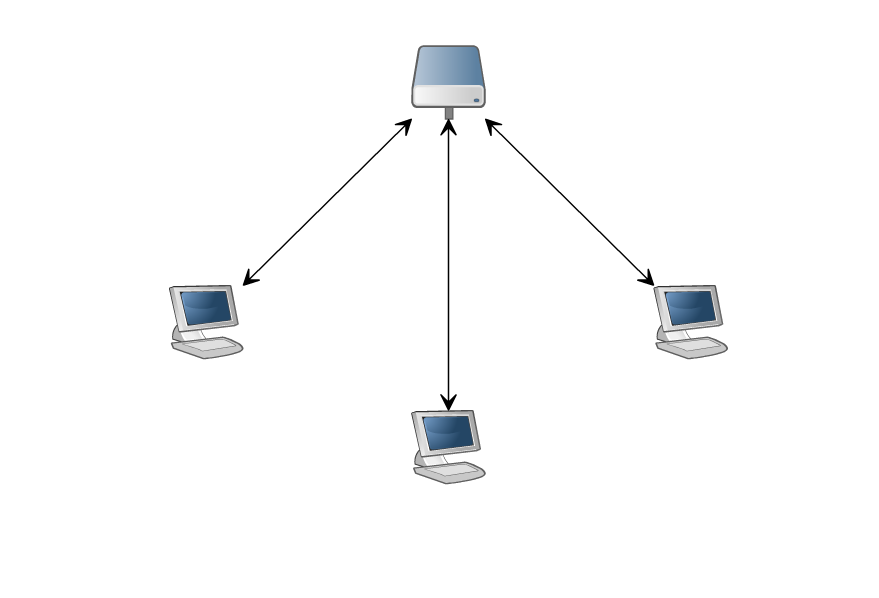
\includegraphics[width=\textwidth]{cs.png}
			\caption{Client-serveur classique}
			\label{fig:archi_cs}
		\end{subfigure}
		~
		\begin{subfigure}[t]{0.3\textwidth}
			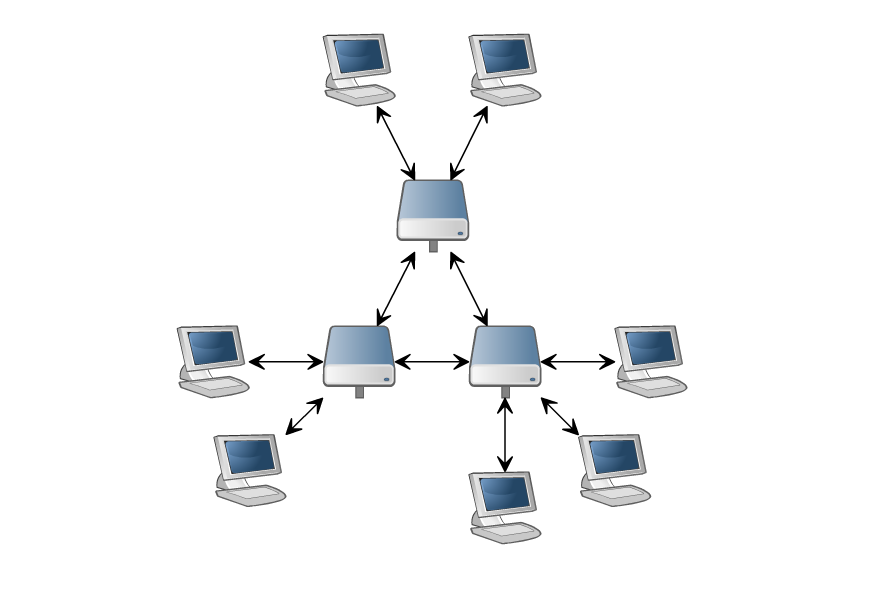
\includegraphics[width=\textwidth]{mcs.png}
			\caption{Multi-serveur}
			\label{fig:archi_mcs}
		\end{subfigure}
		~
		\begin{subfigure}[t]{0.3\textwidth}
			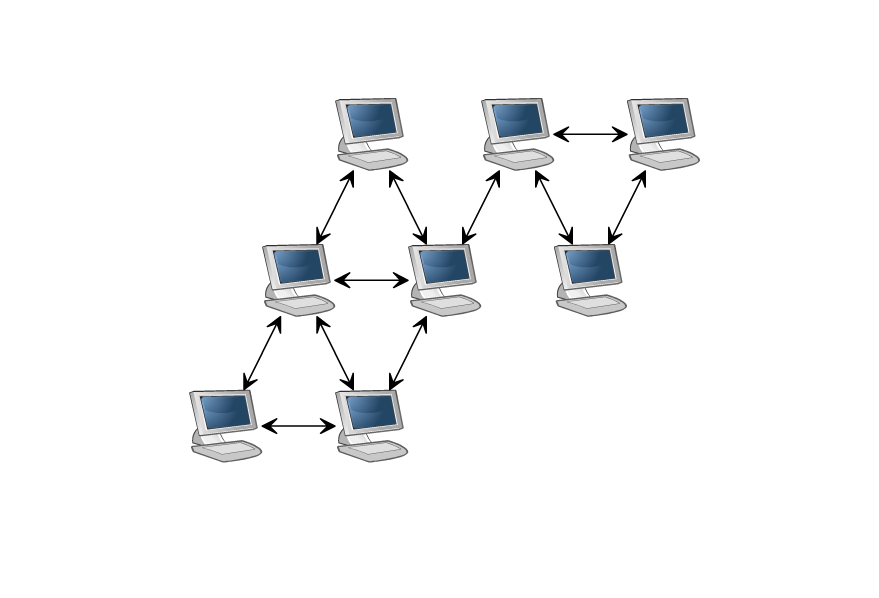
\includegraphics[width=\textwidth]{p2p.png}
			\caption{Pair-à-Pair}
			\label{fig:archi_p2p}
		\end{subfigure}
		\\[0.2cm]
	\caption{Architectures classiques}
	\label{fig:archi}
\end{figure}
Dans l'architecture client-serveur classique, le serveur est responsable de l'état global du monde, il reçoit les mises à jour de la part des clients, calcule le nouvel état et en envoie une copie aux joueurs (\textsc{Figure}~\ref{fig:archi_cs}).
La majeure partie des jeux à succès est basée sur cette architecture.
Les serveurs plus simples peuvent être déployés n'importe où, comme les serveurs de jeux de tir à la première personne ou ceux de Minecraft qui sont très nombreux.

Cette architecture peut également être basée sur de multiples machines pour des plus gros jeux tels que Second Life ou World of Warcraft (\textsc{Figure}~\ref{fig:archi_mcs}).
Ces architectures multi-serveurs se basent sur les partitionnements vus en partie II pour tenir la charge d'un MMOG.

Le serveur BigWorld~\cite{bigworld} est une architecture multi-serveurs qui utilise une grande partie des découpages de la partie précédente (voir \textsc{Figure}~\ref{fig:bigworld}).
Dans cette architecture, chacun des éléments du jeu est séparé en services (login, database...) qui sont hébergés par des machines différentes.
De plus, le monde est découpé en cellules (cell) qui sont des séparations du monde grâce à des rectangles aux côtés alignés qui sont hébergés chacun par une machine.
Comme ces séparations sont dynamiques pour assurer l'équilibrage de charge, les machines sous-utilisées peuvent être arrêtées et leur zones respectives données aux autres machines pour réduire les coûts.
Cela peut également améliorer la durée de vie des machines.

Une technique de proxy peut être mise en place pour permettre de séparer la charge réseau sur différentes machines.
Les machines proxy répliquent l'état du jeu et chacune transmet cet état à un nombre réduit de joueurs (partagé entre tous les proxys).
Ceci tire profit du fait que la connexion inter-machines (réseau local) est bien souvent plus rapide que leur connexion vers l'extérieur (internet).

Le serveur Pikko~\cite{pikko} utilise un serveur écrit en Erlang qui sert de répartiteur de charge entre toutes les machines du serveur de jeu.
C'est ce répartiteur qui décide les transferts de joueurs entre les machines et qui redirige les actions des joueurs vers la bonne machine.
Ceci permettra dans le futur MMOG Warhammer 40000 : Eternal Crusade~\cite{wh40kEC} de faire des batailles comprenant de très nombreux joueurs dans la même zone (plus de 500).
Cette technologie a été testée à l'occasion d'une démonstration nommée Tanks vs. Robots qui a permis d'atteindre un record dans le Guiness Book grâce à 1000 joueurs simultanés~\cite{tanks_vs_robots}.

\begin{figure}[b!]
	\centering
	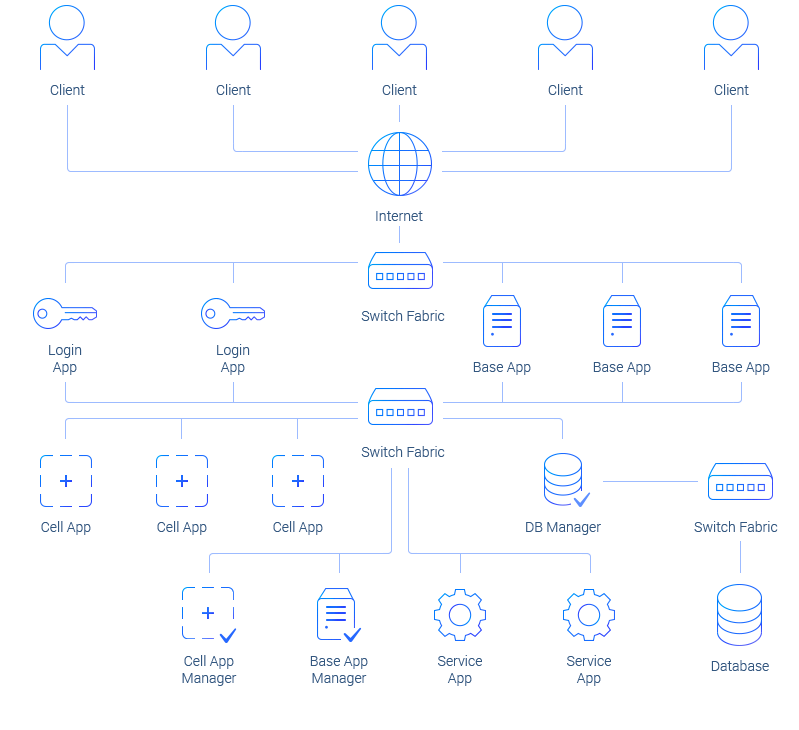
\includegraphics[width=0.7\textwidth]{bigworld.png}
	\\[0.2cm]
	\caption{Fonctionnement du Serveur Bigworld~\cite{bigworld}}
	\label{fig:bigworld}
\end{figure}

\subsection{Architecture Pair-à-Pair}
Un MMOG nécessite d'avantage de ressource pour gérer chacun des nouveaux joueurs se connectant.
Cependant, chacun des joueurs qui se connecte amène également des ressources via son ordinateur.
Les architectures Pair-à-Pair (\textsc{Figure}~\ref{fig:archi_cs}) exploitent ceci en utilisant la puissance de calcul et le réseau des clients pour effectuer les tâches qui s'exécutent normalement du côté du serveur.
Il faut alors intégrer au client du jeu toute la logique du serveur.
Comme chacun des joueurs amène ses propres ressources, le système peut théoriquement passer à l'échelle indéfiniement.

Cette architecture est la problématique la plus étudiée dans le domaine de la recherche pour les architectures de serveurs pour MMOG.
Un des premiers mondes virtuels utilisant l'architecture Pair-à-Pair est Solipsis~\cite{solipsis}.
Dans Solipsis, chaque Pair envoie les mises à jour aux autres pairs situés dans un certain rayon de visibilité.
VON/VAST~\cite{VON}~\cite{VAST} et Voronet~\cite{voronet} utilisent une approche similaire en utilisant une triangulation de Delaunay (et les diagrammes de Voronoi) pour connecter les pairs les plus susceptibles d'échanger de l'information (les plus proches dans le monde virtuel).
Ceci réduit les latences en propageant les mises à jour du monde sous forme de vague.

VoroGame~\cite{vorogame} utilise deux couches de distribution pair-à-pair : une triangulation de Delaunay pour découvrir les voisins et une DHT (table de hachage distribuée) pour stocker les objets du monde.
Colyseus~\cite{colyseus} utilise des rectangles aux bords dynamiques alignés pour répartir la charge entre les clients.

\subsection{Architectures hybrides}
Les architectures hybrides se comportent comme un mélange des deux architectures précédentes.
Des ``Super Peers'' sont élus pamis les joueurs et se comportent comme des serveurs de jeu au sein du maillage de l'architecture Pair-à-Pair.
Ces Super Peers sont choisis pamis les joueurs ayant suffisamment de puissance de calcul et une bonne connexion avec les autres~\cite{super_peer_network}.
Un système utilisant cette architecture est MOPAR~\cite{MOPAR} qui est semblable à VoroGame~\cite{vorogame} mais n'utilisant que les Super Peers pour effectuer les calculs en utilisant des zones fixes.

Cependant, comme ces Super Peers sont responsables de certaines données, il faut les choisir de manière judicieuse.
En effet, un Super Peer peut plus facilement tricher en modifiant les données dont il est le responsable.
Des algorithmes de ``confiance'' peuvent être mis en place pour retirer les joueurs soupçonnés de triches en mettant à contribution des vérifications du côté des autres pairs.
De plus, des machines d'architecture Client-Serveur peuvent faire partie du réseau pour créer une autorité de gestion de la triche.
Il faut remarquer que l'introduction de Super Peers réintroduit le problème de point de chute des architectures client-serveur dans l'architecture Pair-à-Pair~\cite{design_issues_for_p2p_mmog}.

\subsection{Le Game as a Service ou ``cloud gaming''}
Certains industriels commencent à explorer une nouvelle méthode de distribution du jeu vidéo.
Plutôt que de télécharger le client de jeu (qui peut devenir très lourd pour les jeux photoréalistes en 3D), le serveur de jeu envoie directement un flux vidéo du jeu (stream) au joueur qui renvoie en échange les entrées (input) (voir \textsc{Figure}~\ref{fig:gaas}).
Cela permet, par exemple, aux joueurs dotés d'un ordinateur peu puissant de se décharger des calculs graphiques pour exécuter le jeu dans une qualité optimale.
Le nom commercial de cette technique est le ``cloud gaming'' mais un nom correspondant mieux est ``Game as a Service'' car l'architecture nécessite du matériel spécialisé~: elle ne se situe pas chez les fournisseurs de cloud usuels.

Cette méthode, bien qu'intéressante, nécessite une très bonne connexion internet, que de nombreux joueurs ne possèdent pas.
Le service de GaaS de Nvidia (Nvidia Grid~\cite{grid}, service pour leur gamme de tablette Nvidia Shield) impose comme prérequis 40 à 60 ms de ping et 10 Mbps en téléchargement par exemple.
De plus, la charge de calcul graphique et réseau du côté serveur devient bien plus importante qu'un serveur ne partageant que l'état du jeu.
Le matériel spécialisé dans ce type de service est d'ailleurs très cher et peu performant.
Par exemple, Nvidia propose la gamme Nvidia Grid (matériel) avec le modèle K520 qui permet de fournir de 2 à 16 joueurs, en résolution 720p à 30 images par seconde, constaté neuf à 2800\$ le 13/03/2015 chez Amazon~\cite{grid_k520}.
L'investissement est donc important pour le nombre de joueurs que la carte peut fournir et la vidéo fournie n'est pas d'une qualité que l'on aurait avec une carte graphique sur un ordinateur de bureau (1080p et 60 images par seconde) sans encombrer le réseau.

Certains fournisseurs utilisent cette méthode pour diffuser du contenu en local pour l'utilisateur, pour par exemple jouer à un jeu très demandeur en ressources sur un ordinateur beaucoup moins puissant que nécessaire en utilisant la puissance d'un autre ordinateur sur le réseau local, par exemple Steam In-Home Streaming~\cite{steam_inhome}, GamingAnywhere~\cite{gaminganywhere_article} ou StreamMyGame~\cite{streammygame}.
Ceci permet par exemple de jouer sur une télévision à l'aide d'un mini-ordinateur.

\begin{figure}[t!]
	\centering
	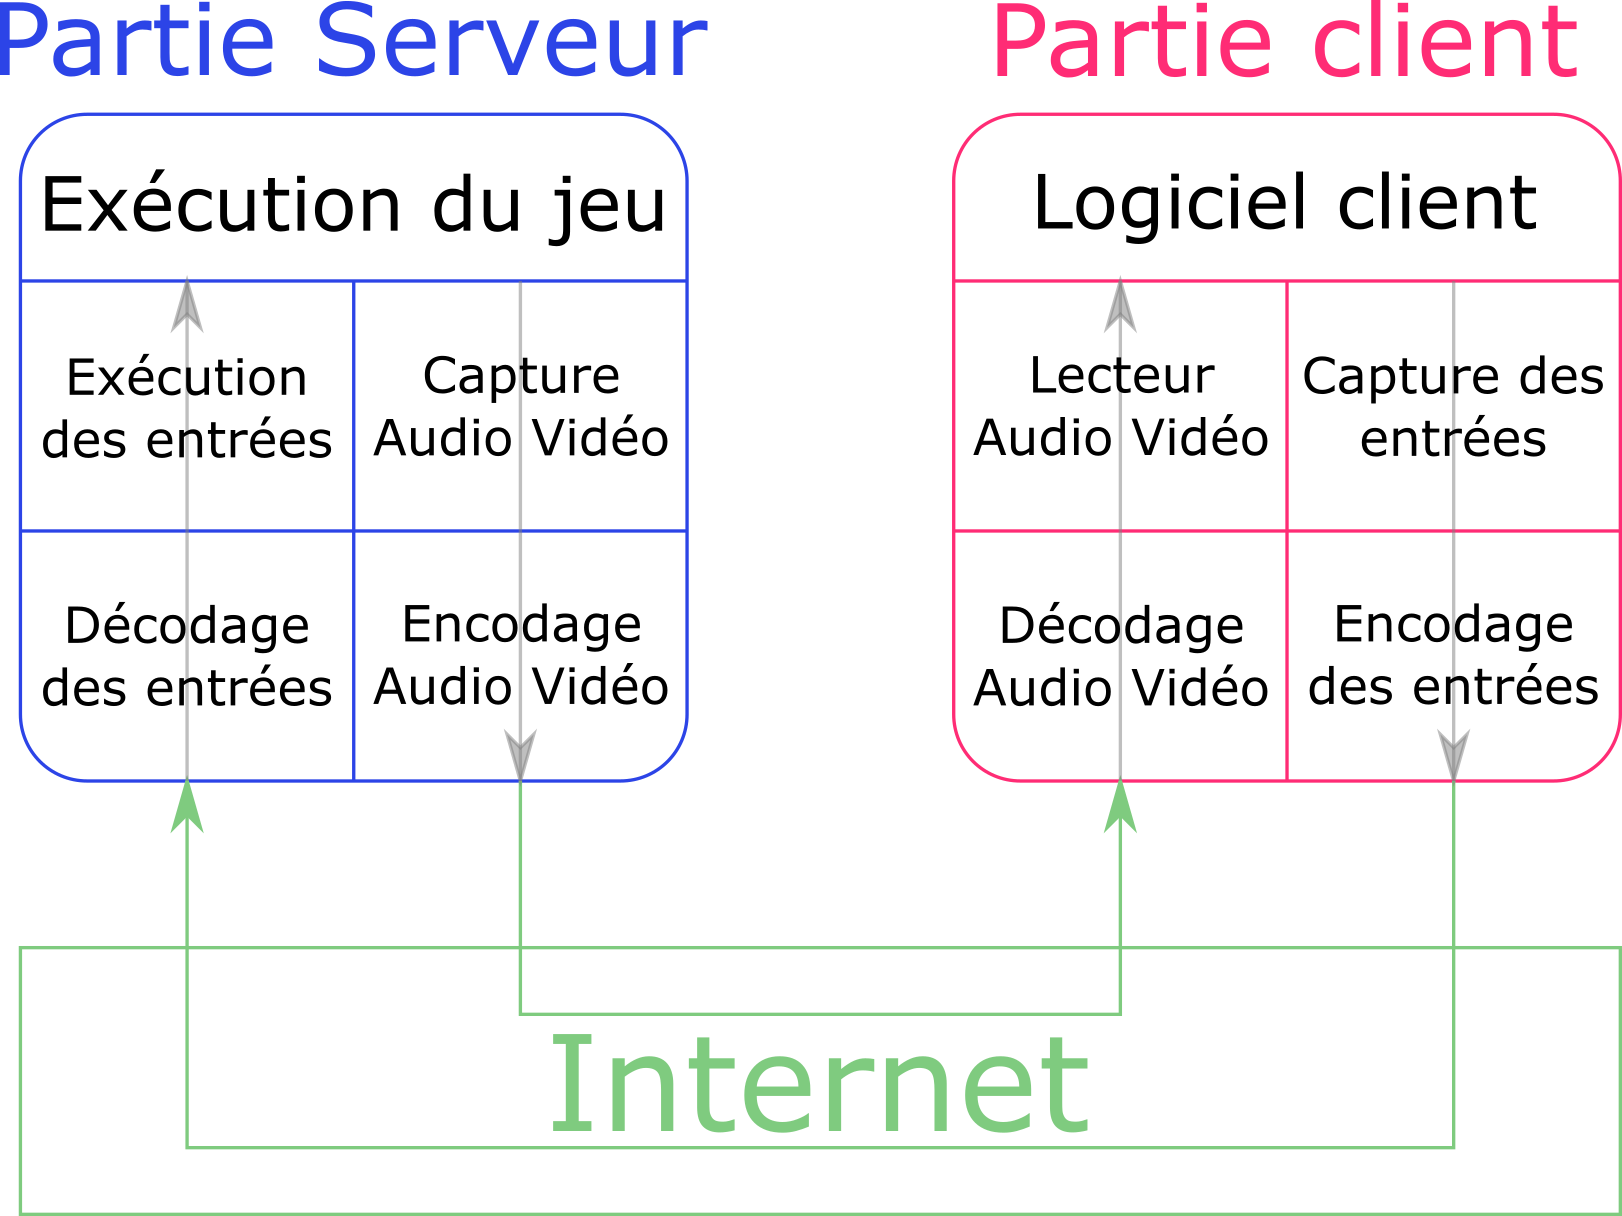
\includegraphics[width=0.5\textwidth]{gaas.png}
	\\[0.2cm]
	\caption{Fonctionnement du Game as a Service}
	\label{fig:gaas}
\end{figure}


\section{Comparaison des architectures}

\subsection{Métriques}

Pour comparer les architectures et les confronter à notre solution, nous allons avoir besoin de métriques quantifiables.
Nous avons sélectionné un certain nombre de métriques présentées dans la suite de cette partie.
Il faut remarquer que, comme notre objectif est de réunir tous les joueurs, cela pourrait entraîner de nouvelles possibilités et des comportements différents des joueurs.
Comme l'architecture que nous proposons n'est pas encore utilisée, des métriques insignifiantes pour les architectures existantes pourraient se révéler importantes durant la suite du stage.

\paragraph{Latence input-résultat\\}
Le facteur déterminant de la jouabilité d'un jeu est la latence entre l'action d'un joueur et le résultat qui s'affiche pour lui à l'écran, surtout dans les jeux d'action rapide type jeu de tir à la première personne~\cite{latency_can_kill}~\cite{latency_and_player_actions_in_online_games}.
Le temps que l'information reçue s'affiche à l'écran n'est pas facilement mesurable et négligeable (60 images par seconde étant affichées à l'écran du joueur).
On considère alors comme latence le temps entre l'émission de l'action du joueur au serveur et la réception d'une mise a jour du monde contenant un acquittement de cette action.
Pour réduire les effets de la latence, le client approxime bien souvent les effets de l'action du joueur et rectifie en cas de divergence lors de la réception suivante de l'état du jeu si nécessaire.
Cependant cette rectification entraîne un phénomène de retour en arrière nuisible à l'immersion du joueur.

\paragraph{Tickrate\\}
Le ``tick'' correspond à un tour de la boucle de simulation de l'état du jeu (récupérer les action des joueurs, les traiter, mettre à jour l'état des objets et renvoyer le nouvel état aux joueurs).
Plus il y a de tick de jeu par seconde (``tickrate''), plus le jeu semblera fluide car les mises à jour de l'état seront plus fréquentes.
Le tickrate est la plupart du temps une donnée fixe car un tick simule une durée fixe d'évolution de l'état du jeu.
Il faut donc éviter des phénomènes de dilatation du temps avec un tickrate qui varie.
Le tickrate a une influence sur la latence input-résultat car le traitement des actions des joueurs est traité pendant chaque tick et le résultat renvoyé à la fin.
Pour éviter de surcharger les clients, le serveur n'est pas obligé d'envoyer à chaque tick un nouvel état du jeu car le client peut effectuer une extrapolation entre les deux états du jeu.
Cela évite de surcharger le réseau avec des modifications mineures.

\paragraph{Charge CPU\\}
La majeure partie de la charge CPU du serveur de jeu n'est pas de calculer les nouveaux états des objets constituant le monde du jeu (traiter les actions des joueurs) car leur portée est limitée et les modifications simples mais de vérifier que ces actions sont autorisées pour éviter la triche.
Cette ressource est le plus souvent le facteur limitant d'un serveur de jeu vidéo, le serveur n'arrivant plus à traiter les requêtes d'actions des joueurs à temps pour garder une expérience de jeu fluide (faisant diminuer le tickrate).
La charge CPU sera mesurée comme le nombre d'opérations à exécuter par seconde, cette mesure ne variant pas avec le modèle de CPU considéré.

\paragraph{Charge Réseau\\}
La charge réseau est une métrique significative car elle est souvent un des facteurs limitants pour le serveur.
En effet, en transposant le problème à d'autres domaines tels que l'hébergement de site internet, le serveur a très peu de charge CPU mais est limité par sa capacité à transférer les pages aux clients.
Il faut aussi remarquer que la bande passante des connexions ADSL des utilisateurs est souvent faible (surtout en upload).
Il faut donc limiter les interactions pour éviter de saturer le réseau des clients pouvant être utilisé pour d'autres domaines plus prioritaires (voix sur IP, télévision par internet...).
Il faut également faire attention à ne pas saturer les connexions inter-serveurs pour que les mises à jour de l'état du jeu puissent se faire.
On différenciera alors vitesse de téléchargement (download) et envoi (upload) pour les machines du serveur et les clients.

\paragraph{Charge Mémoire\\}
La mémoire n'est souvent pas la ressource limitante d'un serveur de jeu vidéo, les entités gérées ayant la majeure partie du temps une emprunte mémoire mineure (coordonnées et états).
Cependant, dans des machines ayant peu de mémoire (par exemple des VM dans le cloud), cela peut devenir un problème.
De plus, si il y a pression mémoire, le système devra ``swapper'' des pages mémoires sur le disque qui est un périphérique très lent comparé à la RAM.
Cela arrive par exemple dans le cas des environnement où le serveur de jeu n'est pas le seul programme à s'exécuter sur la machine.
Cette métrique sera donc pour nous une métrique mineure mais sera tout de même surveillée dans notre solution pour vérifier que cela ne soit pas un facteur la limitant.

\paragraph{Coûts\\}
Héberger son propre serveur de jeu, surtout dans le cas du jeu massivement multijoueur, est cher.
Pour assurer la disponibilité de l'architecture, il faut munir ses machines de multiples entrées électriques et réseau en cas de défaillance.
Dans le cas de multiples machines, il faut également fournir entre autre choses des solutions de refroidissement.
Cela nécessite de la maintenance et une infrastructure qui coûte cher.
C'est pourquoi de nombreuses entreprises se tournent désormais vers le cloud qui offre cette disponibilité.
Cependant, louer des VM dans le cloud, bien que facturées à la minute, peut coûter cher selon l'utilisation que l'on en fait.
Il faut donc faire attention à la manière dont est utilisé le cloud où les coûts pourraient être plus importants que l'hébergement de serveur de type client-serveur.
Il faut également remarquer que le coût des architectures pair-à-pair est nul car c'est la puissance de calcul et le réseau des joueurs qui sont utilisés.
Dans le cloud, c'est le ``temps-machine'' qui est facturé (nombre de machine $*$ temps d'utilisation) ainsi que l'utilisation du réseau (volume de données échangées).
Il faut également remarquer que dans le cloud un réduction est offerte lors de l'utilisation d'une VM une certaine proportion du temps du mois.
Par exemple, une VM utilisée 50\% du mois coûtera moins cher que deux VMs utilisées 25\% du mois.

\subsection{Comparaison}
\paragraph{Game as a Service\\}
La majeure partie du temps, le GaaS n'héberge pas la partie serveur du jeu mais uniquement les vues à distribuer au client.
L'infrastructure peut disposer d'une latence inférieure et d'une bande passante supérieure à la connexion d'un particulier, mais cette architecture génère beaucoup plus de trafic internet à cause du flux continu de vidéo.
Cela nécessite donc une connexion meilleure pour le joueur comparé à une architecture client-serveur classique qui ne partage que les mises à jour des données logiques du jeu (pour World of Warcraft une dizaine de kbps~\cite{mmorpg_network_performance_session_patterns_and_latency_requirements_analysis}).

\paragraph{Pair-à-Pair\\}
De nombreux éditeurs sont réticents à propos de l'utilisation de l'architecture Pair-à-Pair.
Ceci est probablement dû au modèle économique que ce type d'architecture entraîne.
En effet, tout le serveur de jeu se situe dans le code du client ce qui fait qu'il est plus facile pour des personnes de créer un monde de jeu parallèle en modifiant le code du client.
Un jeu massivement multijoueurs avec abonnement n'est donc pas envisageable dans cette architecture car les joueurs peuvent partir sur le monde parallèle et ne plus payer.
De plus, cette architecture entraîne beaucoup plus de développement car le développeur du jeu ne peut pas avoir confiance envers le joueur hébergeant une partie du monde, le joueur pouvant se déconnecter brutalement ou vouloir tricher par exemple.
Cela entraîne donc le développement de plusieurs techniques telles que des mécanismes de réputation ou des mécanismes de stockage du monde persistant sous forme de table de hachage distribuée (DHT).
Il y a de nombreux problèmes de latence dans ce type d'architectures dues à l'absence d'autorité centrale qui entraîne de la synchronisation.
Cette architecture n'est donc pas adaptée aux jeux vidéos rapides (\textit{fast paced game}) comme les jeux de tir à la première personne.

\paragraph{Client-Serveur\\}
La solution majoritairement utilisée actuellement par les éditeurs de MMOG est une solution client-serveur.
Un solution avec une seule machine n'est pas envisageable car la machine sera rapidement saturé, il faut donc opter pour une solution multi-serveurs.
Cependant, cette architecture ne peut pas passer à l'échelle indéfiniment.
Une machine ne pouvant gérer qu'un nombre fini de joueurs, un nombre fini de machines ne peut gérer qu'un nombre fini de joueurs, le nombre de machines n'évoluant pas ou étant limité par l'infrastructure utilisée.
De plus, cela entraîne un unique point de défaillance du jeu car une coupure d'électricité ou d'internet entraîne une coupure du jeu.
Un très gros avantage de ces architectures est au niveau de la distribution des mises à jour du jeu pour les clients.
Comme les clients ne font que recevoir l'état du jeu, toute la logique se situe dans le serveur.
Une mise à jour peut donc être faite uniquement du côté serveur sans mettre à jour le côté client.

\paragraph{Hybride\\}
L'architecture hybride semble un bon compromis entre le Pair-à-Pair et le client-serveur.
Cependant, les Super Peers ou machines de type client-serveur amènent des points de défaillance du jeu dans l'architecture Pair-à-Pair.
De plus, cela suppose qu'il y ait des pairs avec des capacités supérieures qui soient connectés, ce qui peut ne pas être le cas, particulièrement si le MMOG est sur plateformes mobile (téléphones, consoles portables...).
Il faut également remarquer qu'en effectuant une fusion des deux architectures précédentes pour combler les points faibles d'une des architectures, on amène des points négatifs d'une des autres architectures.

\newpage
\subsection{Tableau récapitulatif}
\vspace{1cm}
\begin{center}
	\begin{tabular}{|>{\centering\arraybackslash}m{0.24\textwidth}|*{3}{>{\centering\arraybackslash}m{0.20\textwidth}|}}
		\hline
		
		~&
		Client-Serveur\linebreak(machine unique)&
		Client-Serveur\linebreak(multi-serveur)&
		Pair-à-Pair\\
		
		\hline
		
		Division du monde&
		Triviale&
		Moyenne\linebreak(Facile si statique)&
		Difficile\linebreak(dynamique dans le nombre d'hôtes)\\
		
		\hline
		
		Cohérence du monde&
		Facile&
		Moyenne\linebreak(verrous)&
		Difficile\linebreak(consensus byzantin)\\
		
		\hline
		
		Tolérance aux fautes&
		Aucune&
		Oui si réplication\linebreak(si le cluster est hors ligne, rien n'est disponible)&
		Oui si réplication\linebreak(sinon perte du monde)\\
		
		\hline
		
		Gestion de la triche&
		Facile\linebreak(centralisée)&
		Facile\linebreak(centralisée)&
		Difficile\linebreak(byzantin)\\
		
		\hhline{|*{4}{=|}}
		
		Charge CPU&
		\'Elevée&
		Réduite&
		Chez le client\\
		
		\hline
		
		Charge Réseau&
		Normale&
		Séparée entre les serveur + Communications internes&
		\'Elevée\linebreak(surtout pour les connexions des particuliers)\\
		
		\hline
		
		Complexité de développement&
		Facile&
		Moyenne&
		Complexe\\
		
		\hline
		
		Coûts&
		Normal&
		\'Elevé\linebreak(sur-dimensionnement)&
		Nulle\\
		
		\hline

    Latence&
		Normale&
		Normale&
		\'Elevée\linebreak(connexion mauvaise des particuliers et lenteur des prises de décisions)\\
		
		\hline
	\end{tabular}
\end{center}
\vspace{0.8cm}

\subsection{Notre solution : le cloud}
On peut remarquer dans le tableau récapitulatif que la méthode la plus avantageuse se situe au niveau de l'architecture Client-Serveur.
Cependant, l'architecture Pair-à-Pair a l'avantage d'être très tolérante aux fautes et de distribuer les charges CPU et Réseau.

Dans ce rapport, nous proposons une autre solution qui n'a pas encore été adoptée par les grands éditeurs de jeux vidéo.
En effet, pour adresser le problème du nombre limité de machines dans une architecture client serveur, on se propose d'utiliser des VM dans le cloud qui, si hébergées chez de grands fournisseurs du type Google Cloud~\cite{google_cloud} ou Amazon EC2~\cite{amazon_ec2}, sont virtuellement en nombre infini (les fournisseurs de ces services ayant des très grands datacenters à travers le monde).
Les fournisseurs de ces services garantissent une certaine qualité de service telle que la disponibilité (aux alentours des 99\% dans la majeure partie des services grâce à de nombreuses alimentation électriques et onduleurs ainsi que plusieurs fournisseurs d'accès à internet).

L'architecture cloud permet, en théorie, de passer à l'échelle indéfiniment car il suffit de faire apparaître de nouvelles VM en cas de surcharge du serveur de jeu.
Pour ce faire, cette architecture utilise les mêmes types de partitionnement que les autres architectures vues dans la partie précédente.
Chaque VM est donc responsable d'une certaine partie du monde qui évolue en fonction de la charge de celle-ci.

Cependant, on peut remarquer que pour limiter le nombre de joueurs dans une même zone, la majeure partie des jeux utilisent le sharding pour limiter le nombre de joueurs sur un même serveur.
On remarque donc que, bien que tous les joueurs jouent au même jeu, les joueurs ne jouent pas forcément ensemble.
Dans ce stage, nous allons nous intéresser à la consolidation de cet univers virtuel et nous n'allons donc pas utiliser le sharding.

Il faut cependant remarquer que louer des VMs dans le cloud peut coûter très cher, surtout si ces VMs se retrouvent sous-utilisées et nombreuses.
En effet, la location de ce genre de machine se faisant à la minute, il est utile de bien dimensionner les VMs pour optimiser l'argent dépensé dans le serveur de jeu.
Il faut également remarquer que de nombreux services réduisent le prix des machines si elles sont utilisées plus qu'un certain pourcentage dans le mois.
Il faudra donc faire en sorte que l'architecture utilise un nombre réduit de VMs pour ainsi en optimiser le coût.



\section{Simulation}
Pour nous permettre d'expérimenter ces architectures nous allons adopter une approche par simulation.
La simulation présente de nombreux avantages, notamment le fait de pouvoir accélérer le temps.
La simulation étant déterministe, on peut par ailleurs rejouer des scénarios qu'il serait impossible de rejouer par expérimentations sur plateformes réelles (perturbations dans le réseau, par exemple latence).
De plus, la simulation peut s'exécuter sur des machines moins puissantes que celles simulées.
Enfin, la simulation est automatisable et permet d'éviter d'avoir à réunir des personnes réelles jouant au jeu pour tester les algorithmes qui seront implémentés dans le système contrairement à de l'expérimentation.

Comme la simulation est compliquée à réaliser, nous allons nous baser sur un c\oe{}ur de simulation déjà existant et développer notre solution par dessus.
Nous n'aurons donc pas à simuler le temps qui s'écoule, le réseau et le CPU dans la simulation mais juste à développer un outil permettant de tester des algorithmes et de mesurer leur efficacité en utilisant les métriques citées plus haut.
Pour permettre au simulateur d'être utilisé pour une grande variété de jeux, il sera également nécessaire de fournir une couche d'abstraction sur laquelle le simulateur se basera.

\subsection{Choix du simulateur}
De nombreux simulateurs existent mais utilisent différents niveaux d'approximation.
Une simulation trop fidèle demanderait beaucoup de ressources et s'exécuterait très lentement.
Inversement, une simulation trop peu fidèle entraînerait des incohérences au niveau des résultats et certains effets de bord ne seraient plus visible (congestion TCP, effet de trafics croisés...).
Trouver un bon compromis est donc important pour effectuer notre simulation.

Comme la réduction de l'encombrement réseau est important dans notre architecture, il faut que le réseau soit simulé de façon correcte et sans trop d'approximations.
Un simulateur tel que PeerSim~\cite{peersim} n'est donc pas pertinent car il n'y a aucune gestion du débit des connexions.
En effet, dans ce type de simulateur, un client peut recevoir plus de paquets que sa connexion ne pourrait le supporter par exemple.

Une autre partie importante du simulateur est la capacité à gérer les architectures de type cloud, c'est à dire gérer un nombre de serveurs dynamique (et théoriquement infini) de machines virtuelles.
Dans certains clouds, la puissance des VMs peuvent également varier au cours du temps, les VMs pouvant être relocalisées ou redimensionnées pendant l'exécution.

Nous avons décidé d'utiliser Simgrid~\cite{simgrid} qui est un simulateur permettant de simuler de nombreuses architectures, dont le cloud en fournissant une interface de type libvirt pour gérer les VM.
Il dispose aussi d'une interface de type POSIX ou MPI pour le développement des applications simulées.
Simgrid utilise une simulation rapide mais réaliste du réseau, modélisant par exemple les effets de bords de TCP.
Simgrid possède des outils de visualisation graphique permettant de voir l'évolution des ressources.
Un module permet également de surveiller les modifications des données de l'application et de générer des traces utilisables pour nos propres outils de visualisation.

\subsection{Simulation des joueurs}
Dans notre simulation, le mouvement des joueurs et leur nombre influent grandement sur la gestion des VMs dans le cloud et l'efficacité des algorithmes s'y rattachant.
Pour plus de réalisme, il faudra donc que notre simulateur soit capable d'exécuter des traces de déplacement de personnes déjà existantes.
Cela permet d'avoir une idée du comportement sur un cas d'utilisation réel du système.

Cependant, se baser uniquement sur des traces existantes entraîne un biais dans la simulation.
En effet, peu de simulations différentes sont possibles et il faut remarquer que ces traces correspondent à une exécution bien précise et pourrait ne pas mettre en avant des comportements particuliers ou, à l'inverse, ne représenter qu'un comportement ponctuel et particulier des joueurs.
Pour nous permettre de faire des expérimentations plus variées, il faut générer des traces réalistes de joueurs qui pourront être rejouées pour comparer les algorithmes.
L'intérêt est de pouvoir faire varier les paramètres de déplacement pour tester les limites du système.
De plus, due à la limitation du passage à l'échelle des architectures existantes, le nombre de joueurs des traces existantes est faible comparé à l'échelle requise par nos expérimentations.

Le stage s'est donc naturellement orienté d'abord vers la génération de ces traces qui sont un travail préliminaire pour la simulation de l'architecture de serveur, la répartition sur les serveurs étant fortement dépendante de la répartition des joueurs.



\section{Conclusion}
L'objectif visé par une architecture de serveur de jeu massivement multijoueurs dans le cloud est de réunir tous les joueurs d'un même jeu dans un même monde simulé sans bordures pour permettre une immersion plus grande dans le jeu, contrairement à la séparation en groupes distincts (\textit{Sharding}) effectué habituellement.
Il faut cependant remarquer que le sujet dépasse du cadre du stage, qui est un travail préliminaire pour la recherche dans le domaine.
Un sujet de thèse, que j'effectuerai a la fin de ce stage, a donc été créé pour effectuer la recherche sur des algorithmes efficaces de répartition et de provisionnement entre les machines.
Il faudra également comparer l'efficacité ces algorithmes aux autres architectures existantes pour vérifier que cette architecture fonctionne mieux et coûte moins cher.

La séparation en zones de l'ensemble du monde de jeu est donc nécessaire pour éviter le \textit{Sharding}, chaque serveur étant responsable d'une zone.
La séparation étant dynamique et dépendant de la densité en joueurs, elle est donc fortement dépendante de la répartition des joueurs.
Nous avons donc eu besoin d'un générateur de traces réalistes de mouvements de joueurs (SpringVisualizer) pour tester les différents algorithmes de répartition.
Les traces générées par SpringVisualizer nous permettrons de tester ces algorithmes, à la fois dans des cas ``normaux'', mais aussi dans des cas extrêmes.
SpringSimulator utilise donc ces traces pour simuler l'architecture des serveurs et les clients.
L'objectif de la thèse est de fournir un middleware pour la gestion de serveurs de jeu dans le Cloud, comme RTF~\cite{rtf_middleware_development} le fait pour les environnements multi-serveurs.
La gestion des fautes (franches ou byzantines) sera envisagée dans la suite de la thèse.
Le simulateur Simgrid~\cite{simgrid}, bien qu'efficace, manque peut-être encore de fonctionnalités pouvant servir à l'élaboration de ce simulateur.
Il pourra donc être nécessaire durant la thèse d'effectuer des ajouts à Simgrid.


\bibliographystyle{plain}
\bibliography{references}
\end{document}
